\section{Modelagem}
Trataremos o problema descrito em sua discreta, i.e., dado um valor $\delta$ definimos uma malha quadriculada que cobre toda a regi\~{a}o de interesse como na Figura~\ref{fig:malha_quad}.
\begin{figure}[!htb]
    \centering
    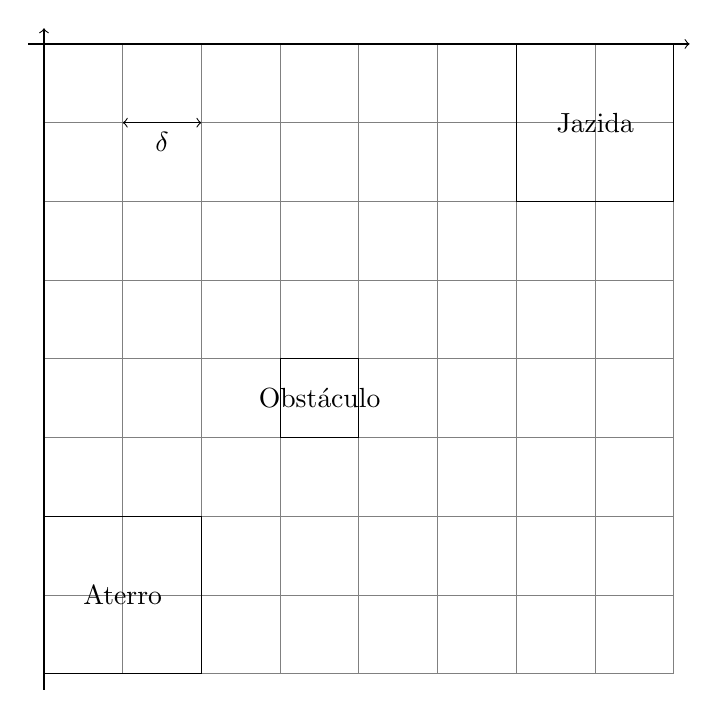
\begin{tikzpicture}
        \draw[color=gray] (0,0) grid (8,8);
        \draw[->] (-.2,8) -- (8.2,8);
        \draw[->] (0,-.2) -- (0,8.2);

        \draw (0,0) rectangle (2,2) node[midway]{Aterro};
        \draw (3,3) rectangle (4,4) node[midway]{Obst\'{a}culo};
        \draw (6,6) rectangle (8,8) node[midway]{Jazida};

        \draw[<->] (1,7) -- (2,7) node[midway, below]{$\delta$};
    \end{tikzpicture}
    \caption{Ilustra\c{c}\~{a}o da malha quadricular sobre a regi\~{a}o de interesse.}
    \label{fig:malha_quad}
\end{figure}

Ao utilizar a malha quadriculada podemos definir a dist\^{a}ncia entre dois quadrados da malha de pelo menos tr\^{e}s maneiras diferentes:
\begin{enumerate}
    \item $d_l$, que \'{e} a menor dist\^{a}ncia entre qualquer dois pontos dos quadrados,
    \item $d_u$, que \'{e} a maior dist\^{a}ncia entre qualquer dois pontos dos quadrados, e
    \item $d_c$, que \'{e} a dist\^{a}ncia entre os centros dos quadrados.
\end{enumerate}
Na Figura~\ref{fig:dist_malha} \'{e} ilustrado cada uma das dist\^{a}ncias acima descrita.
\begin{figure}[!htb]
    \centering
    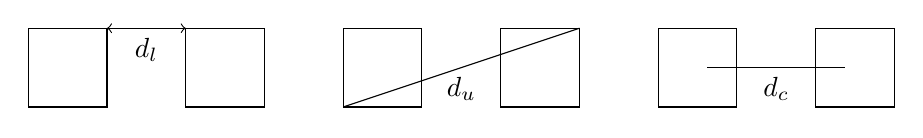
\begin{tikzpicture}
        \draw (0,0) rectangle (1,1);
        \draw (2,0) rectangle (3,1);
        \draw[<->] (1,1) -- (2,1) node[midway, below]{$d_l$};

        \draw (4,0) rectangle (5,1);
        \draw (6,0) rectangle (7,1);
        \draw (4,0) -- (7,1) node[midway, below]{$d_u$};

        \draw (8,0) rectangle (9,1) node[midway](A){};
        \draw (10,0) rectangle (11,1) node[midway](B){};
        \draw (A) -- (B) node[midway, below]{$d_c$};
    \end{tikzpicture}
    \caption{Ilustra\c{c}\~{a}o das dist\^{a}ncias entre quadrados da malha.}
    \label{fig:dist_malha}
\end{figure}

Quanto ao obst\'{a}culo
